\section*{Figures}
\subsection*{Figure legends}

\noindent Figure 1. Global map of Large Marine Ecosystems (LMEs) and
high seas areas (ovals) showing the number of stock assessments
present in the database for each area. This map illustrates the limited
coverage of available stock assessments.\\

\noindent Figure 2. Comparison of the taxonomic diversity of marine
species as provided by FishBase (top panel), the coverage of catch
data as provided by the Sea Around Us Project (SAUP) database (middle
panel) and the new RAM Legacy database (bottom panel). To facilitate the
identification of the taxonomic groups that are not presented in the catch
and assessment data, the FishBase branching pattern of the spoked dendrogram is
maintained to generate the other two dendrograms.\\ 

\noindent Figure 3. Orca plots showing the temporal coverage of (A)
catch/landings, (B) spawning stock biomass and (C) recruitment. The
temporal coverage for individual assessments is represented by thin
alternating black and grey horizontal lines in the main panels. Orca
plots are named because their distinctive shape is uncannily similar
to the individually-identifiable nicked and notched dorsal fins of
killer whales (orcas). Thick horizontal lines at the base of each main
panel represent the time periods which are present in 90\% (black) and
50\% (grey) of all series for that data type.  Subfigure histograms
contain the frequency of occurrence of the various timespans without
reference to time period. Solid and long-dash vertical lines within
the subfigures represent the median,
2.5\% and 97.5\% quantiles, respectively.\\

\noindent Figure 4. Current exploitation rate versus current biomass
for 241 individual stocks. Exploitation is scaled relative to that
which should allow maximum sustainable yield ($U_{msy}$); biomass is
scaled relative to $B_{msy}$. Shades of grey indicate probability of
occurrence as revealed by a kernel density smooth function. Solid
circles indicate $B_{msy}$ and $U_{msy}$ that were obtained directly
from assessments; open circles indicate that they were estimated from
surplus production models. This figure is an updated version of Fig 3B
from \citet{Worm:etal:2009:science}.
\\

\noindent Figure 5. Current exploitation rate versus biomass for
individual stocks grouped by management unit. The panel labelled
``Atlantic'' comprises ICCAT and NAFO. Plot details as in
Figure 6.\\


\newpage
\subsection*{Figures}

\begin{landscape}
\begin{figure}
\begin{center}
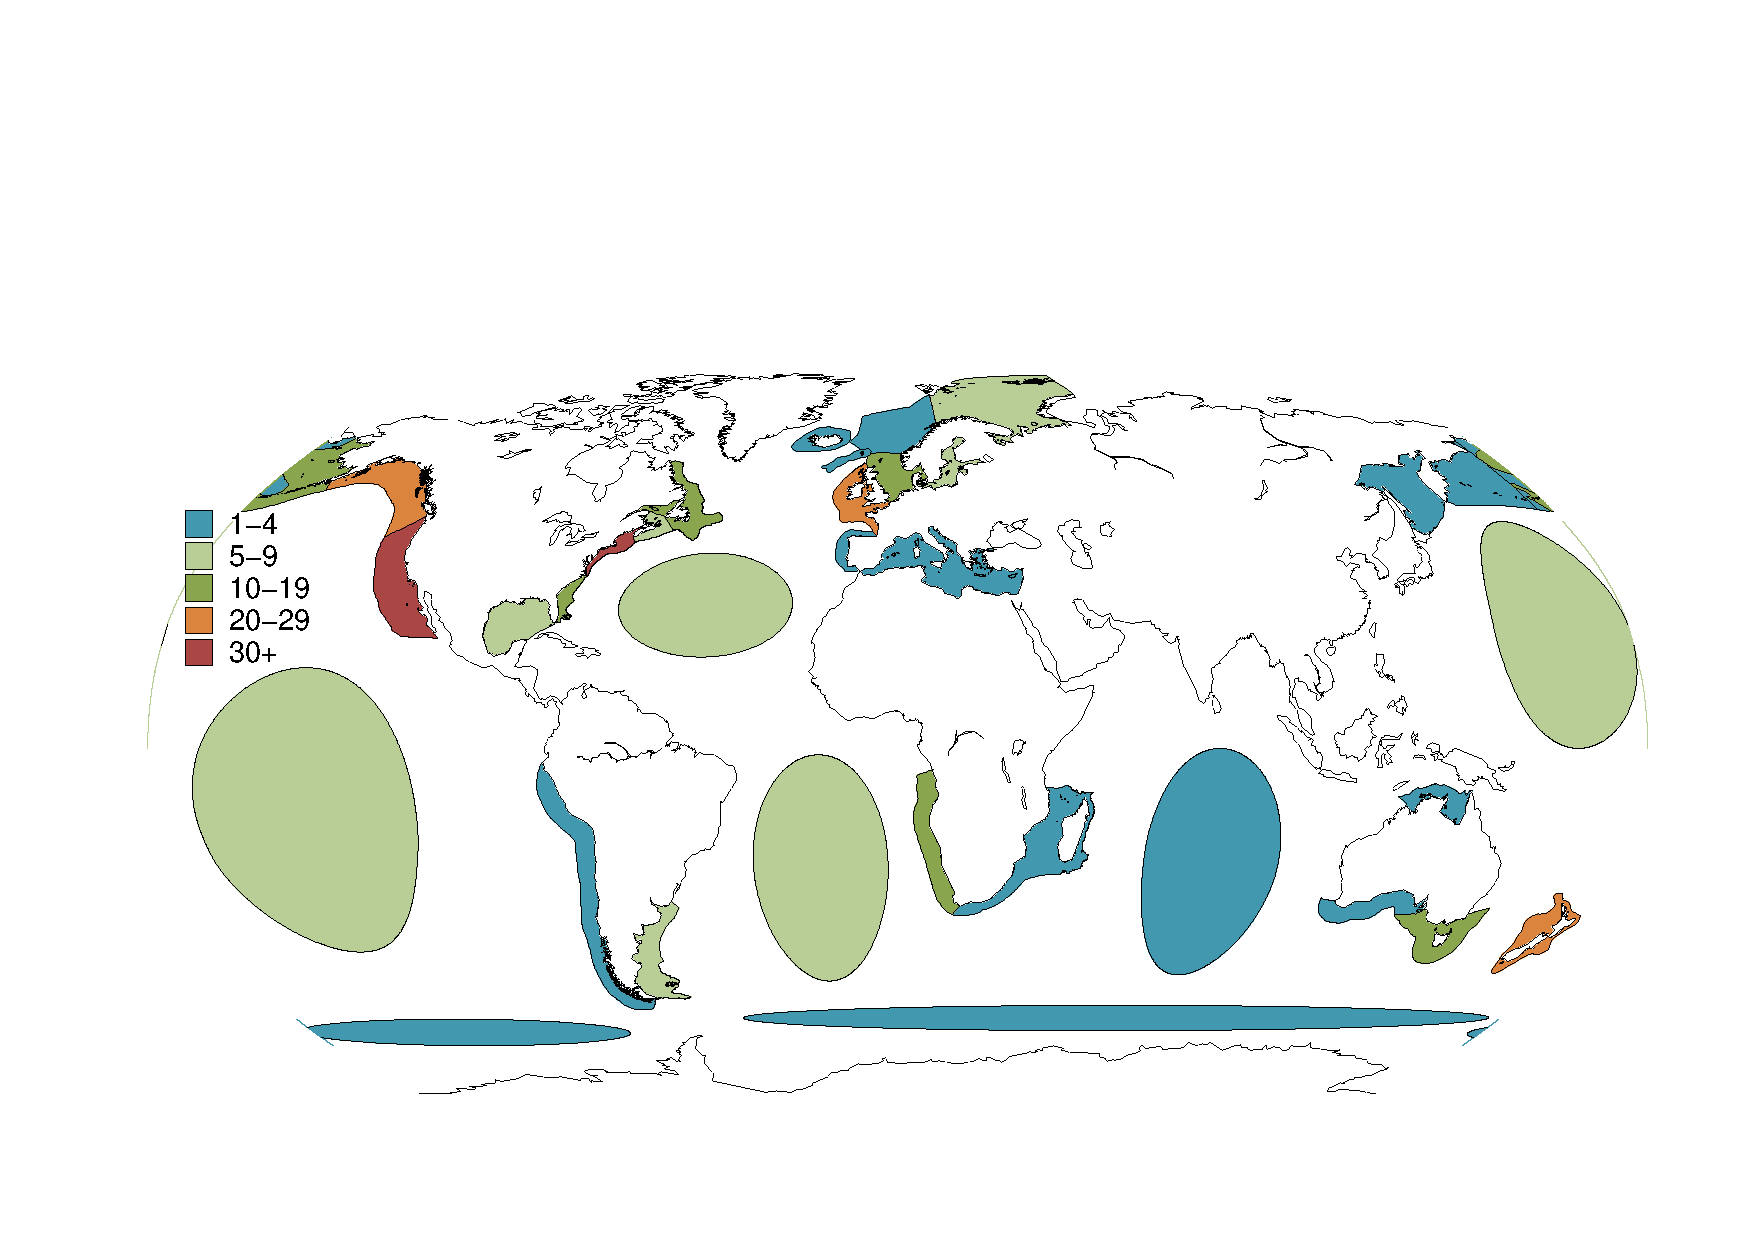
\includegraphics[width=9in]{/home/srdbadmin/srdb/projects/fishandfisheries/GMT/stocks-byLME.pdf}
\end{center}
\caption{ }\label{fig:lmes}
\end{figure}
\end{landscape}


\begin{figure}
\begin{center}
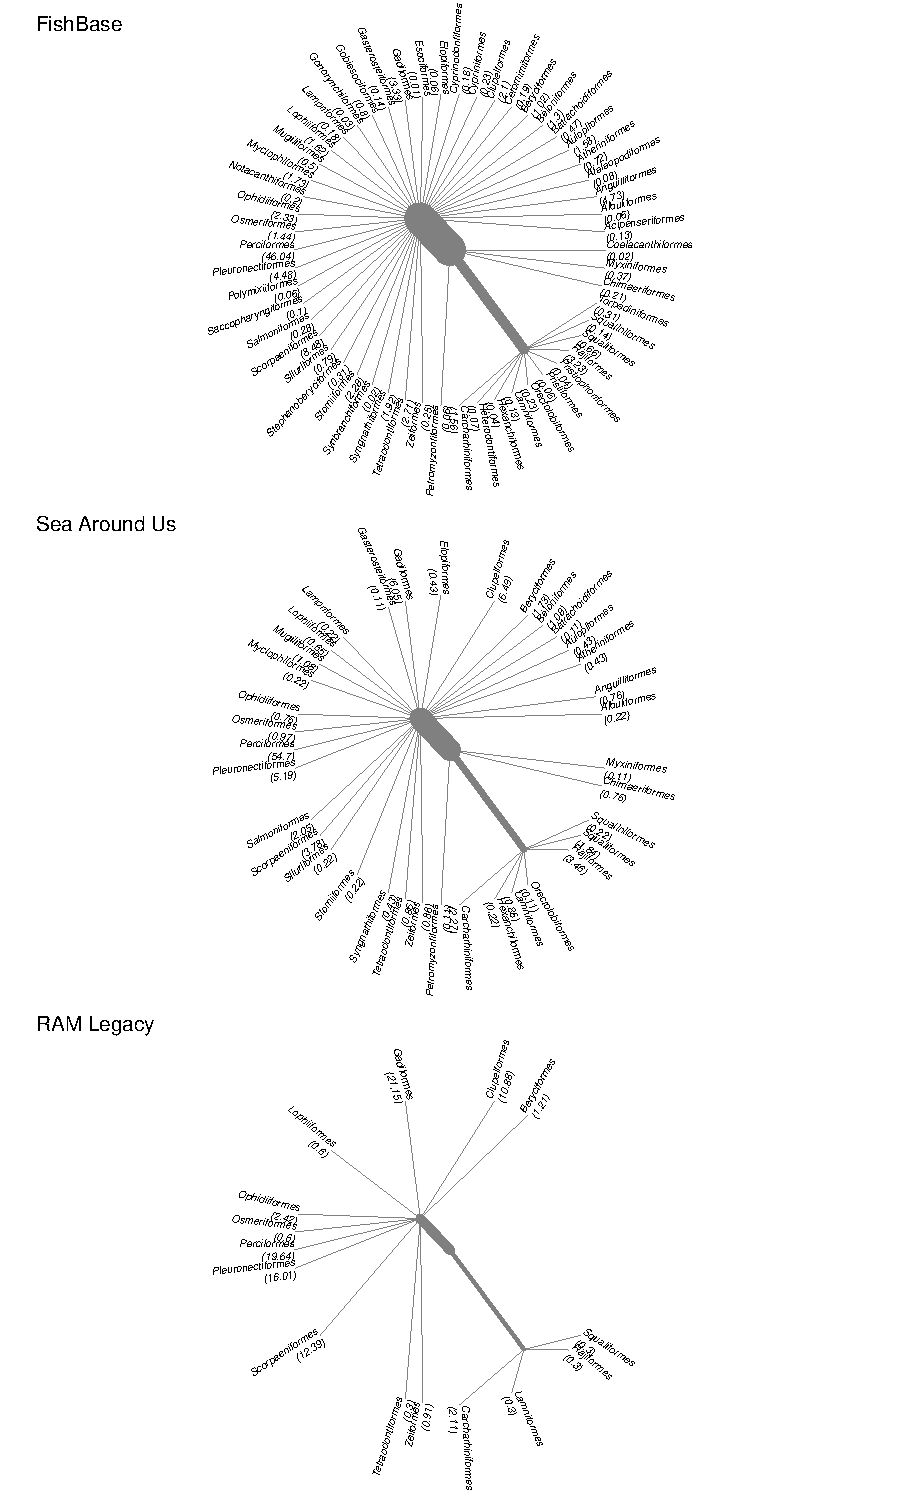
\includegraphics[height=8.5in]{/home/srdbadmin/srdb/projects/fishandfisheries/R/first-review/three-panel-phylo.pdf} % fishbase_saup_two_panel_phylo.pdf}
\end{center}
\caption{ }\label{fig:taxo:threepanel}
\end{figure}



\begin{landscape}
\begin{figure}
\begin{center}
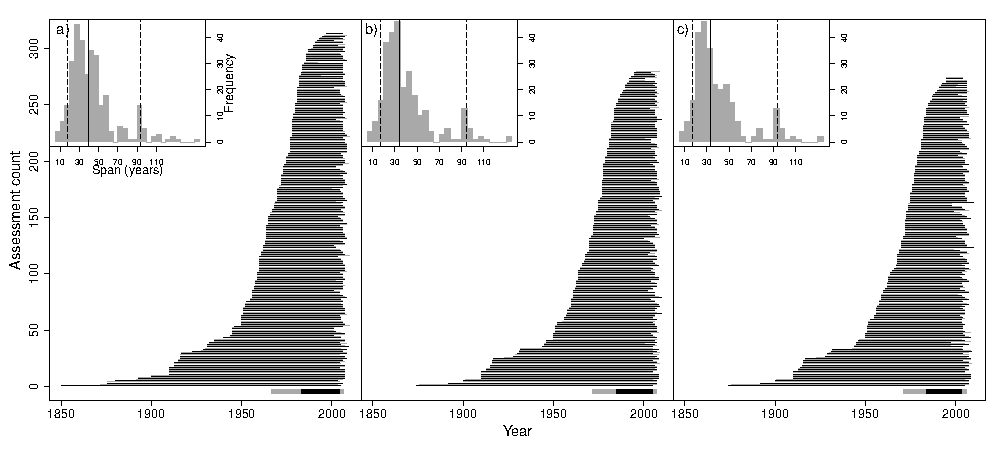
\includegraphics[width=8in]{/home/srdbadmin/srdb/projects/fishandfisheries/R/first-review/orca-plot.pdf}
\end{center}
\caption{ }\label{fig:orca}
\end{figure}
\end{landscape}

\begin{figure}
\begin{center}
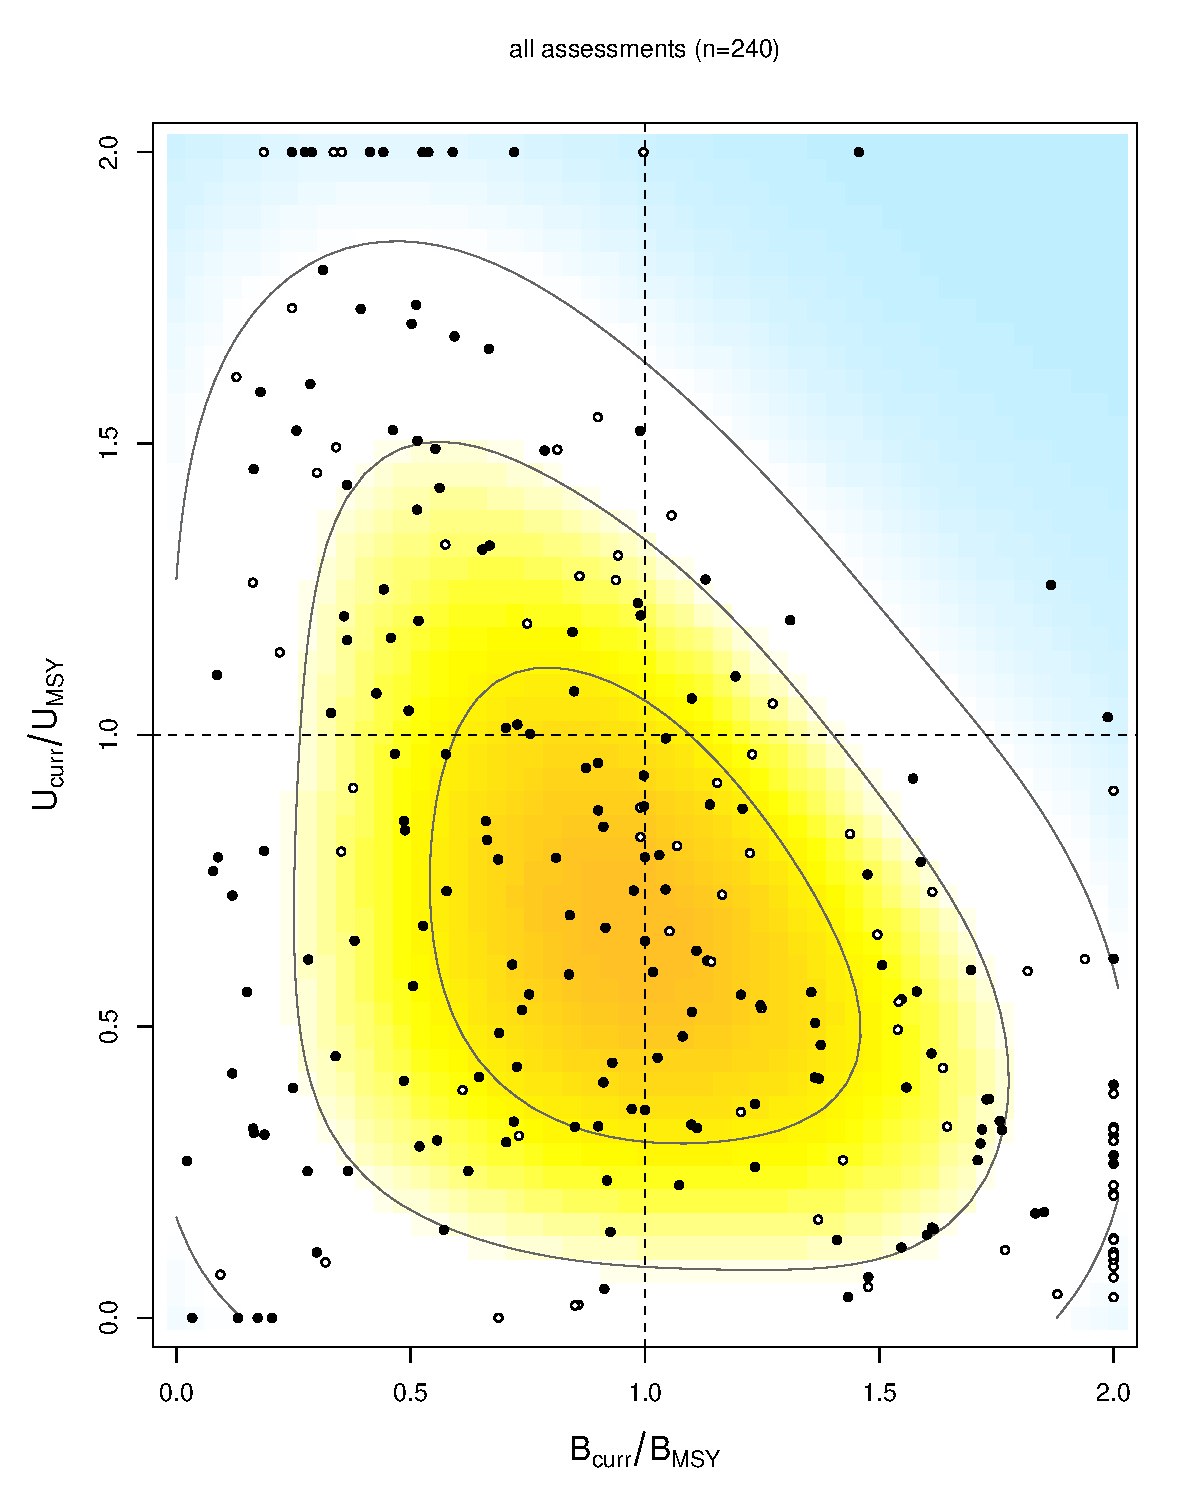
\includegraphics[width=15cm]{/home/srdbadmin/srdb/projects/fishandfisheries/R/first-review/friedegg-single.pdf}
\end{center}
\caption{ }\label{fig:friedegg}
\end{figure}

\begin{figure}
\begin{center}
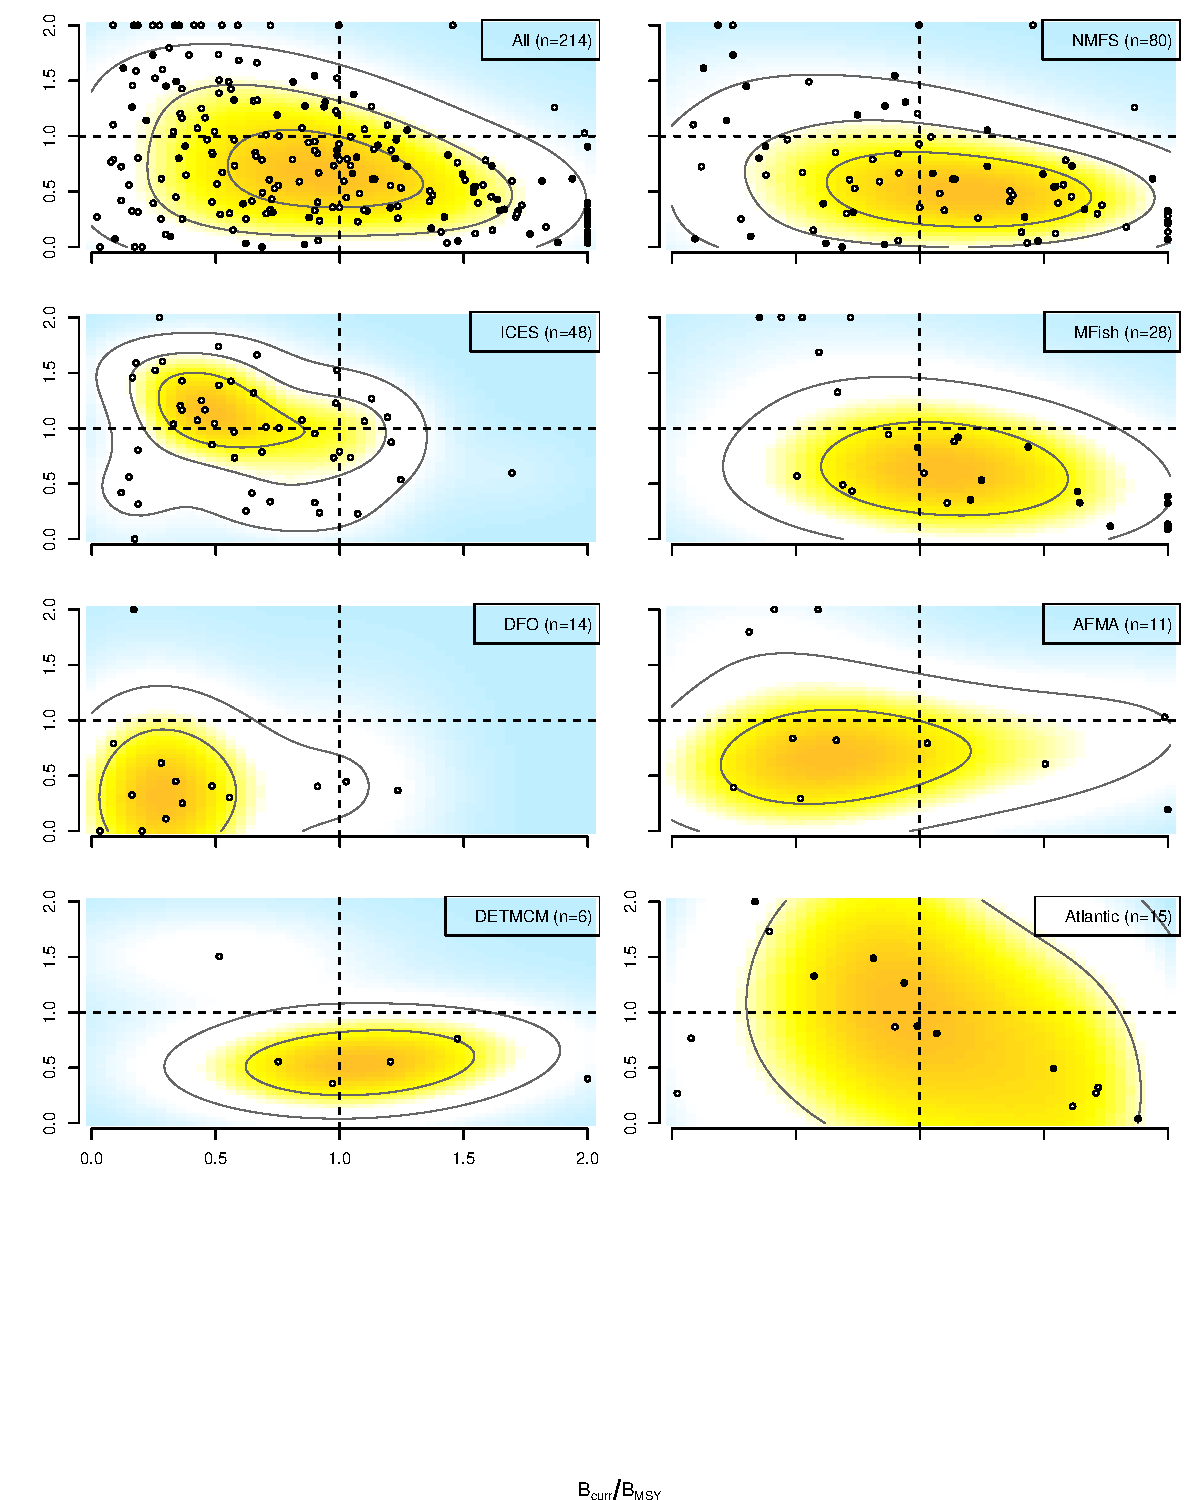
\includegraphics[width=15cm]{/home/srdbadmin/srdb/projects/fishandfisheries/R/first-review/friedegg-bymgmt.pdf}
\end{center}
\caption{ }\label{fig:friedeggmgmt}
\end{figure}

